

% **************************************************
% Load and Configure Packages
% **************************************************

\documentclass[
10pt,						% font size
paper=A4,					% paper size --> A4 is default in Germany
twoside=true,				% onesite or twoside printing
openright,					% doublepage cleaning ends up right side
chapterprefix=true,			% prefix for chapter marks
headings=normal,			% size of headings
%bibliography=totoc,			% include bib in toc
%listof=totoc,				% include listof entries in toc
titlepage=on,				% own page for each title page
captions=tableabove,		% display table captions above the float env
draft=false,				% value for draft version
]{report}
\author{Andre Sealy}
\usepackage{amsmath, amsfonts, amssymb, amsthm,}
\usepackage{tikz}
\usetikzlibrary{matrix,positioning}
\tikzset{bullet/.style={circle,fill,inner sep=2pt}}
\usepackage{braket}
\usepackage{bbold}
\usepackage[margin=1.0in]{geometry}
\usepackage{mathtools}
\usepackage{xfrac}
\usepackage{xcolor}
\newcommand{\lam}{$\lambda$}
\usepackage{pgfplots}
\tikzset{My Style/.style={samples=100, thick}}
\usepackage{graphicx}
\usepackage{bbold}
\usepackage{pgfplots}
\usepackage{setspace}
\usepackage{enumerate}
\usepackage{hyperref}
\usepackage{array}
\usepackage{listings}
\usepackage[official]{eurosym}
\usepackage[shortlabels]{enumitem}
\usepackage{booktabs}
\usepackage{floatrow}
\floatsetup[table]{capposition=top}
\usepackage{xcolor}
\usepackage{appendix}
\hypersetup{
	colorlinks,
	linkcolor={red!50!black},
	citecolor={blue!50!black},
	urlcolor={blue!80!black}
}
\makeatletter
\def\amsbb{\use@mathgroup \M@U \symAMSb}
\makeatother

\onehalfspacing

\begin{document}
	
	% --------------------------
	% rename document parts
	% --------------------------
	

	% --------------------------
	% Front matter
	% --------------------------
	\pagestyle{empty}				% no header or footers
	% !TEX root = ../thesis-example.tex
%

% ------------------------------------  --> main title page
\begin{titlepage}
    \centering
\vspace*{1cm}
{ 
\includegraphics[width=10cm]{images (2).png}}\\[1cm]

{\LARGE \textbf{Comparing Methodologies for Pricing Barrier Options}}\\[1cm]

\textbf{FE 620: Pricing and Hedging}\\
Final Project\\[0.5cm]

\textbf{Written By:}{}\\
Amod Lamichhane \\[0.5cm]
Andre Sealy \\[0.5cm]
Jeffrey Gebauer \\[0.5cm]
\date{\large Date Last Edited: \today}
\end{titlepage}
		% INCLUDE: all titlepages
	\cleardoublepage
	\tableofcontents
	\cleardoublepage
	% --------------------------
	% Body matter
	% --------------------------+
%	% !TEX root = ../thesis-example.tex
%


\chapter{Introduction}
\everymath{\displaystyle}
\captionsetup[figure]{font=large}
 % INCLUDE: introduction
	% !TEX root = ../thesis-example.tex
%
\chapter{Barrier Options}
\section{Background}
Barrier options are path-dependent options with price barriers; their price depends on whether the underlying asset's price reaches a certain level during a specific period. Various types of barrier options regularly trade over-the-counter and have done so since 1967 \cite{JohnRubinstein1985}. These exotic options were developed to address the specific hedging concerns and market conditions that European and American options failed to accommodate. Barrier options are very popular for their risk-management solutions, as they allow investors and institutions to take various positions with very specific levels of protection.

As financial markets continued to evolve in the 1990s, barrier options became more standardized and accessible to the financial population. Derivative exchanges and financial institutions offered barrier options on various underlying assets, such as commodities, currencies, and interest rates. The 2008 global financial crisis sparked a renewed interest in derivative products for their risk-management capabilities, and barrier options remained one of the best products for their ability to tailor risk profiles to specific market conditions. In addition, computational tool advancements make pricing these options more manageable, thereby increasing the accessibility to market participants. This report will outline the many analytical and computational tools for pricing barrier options.

\section{Options Payoffs}
For some background, we will briefly discuss the attributes of a vanilla option. A call option gives the holder the right, but not the obligation, to buy a particular number of the underlying assets in the future for a pre-agreed price known as the strike price (put options give the holder the right, but not the obligation, to sell). While European options can only be exercised on the expiration date, American options allow the holder to exercise at any time on or before the expiration date. We will focus on European options throughout this research report.

Let $S$ be the price of an underlying asset and $K$ be the strike price, where $S,K\in\amsbb{R}^+$. Then the payoff for a vanilla call option, $V_c$, is given by the following
\begin{equation}\label{eq:vanilla_call}
	V_c(S,T)=\begin{cases}
		S_T-K  & \text{if }S_t>K,\forall t\in[0,T) \\
		0 & \text{otherwise}
	\end{cases}
\end{equation}
Likewise, the payoff for a vanilla put option, $V_p$, derived by the following:
\begin{equation}
	V_p(S,T)=\begin{cases}\label{eq:vanilla_put}
		0 & \text{if }S_t>K,\forall t\in[0,T) \\
		K-S_T  & \text{otherwise}
	\end{cases}
\end{equation}
These formulas drive our intuition of how both vanilla and exotic options can be priced.
\section{Barrier Option Payoffs}
As we can see, the payoff of a vanilla option depends only on the terminal value of the underlying asset. However, an exotic option, such as a barrier option, is very different. Its price is determined by whether the underlying asset's price reaches a certain level during a specific period. Barrier options differ from standard vanilla options in several ways. 

First, they match the hedging needs more closely than standard options; second, premiums for barrier options are typically lower than vanilla options; and finally, the payoff of a barrier option matches beliefs about the future behavior of the market. These features benefit many different types of investors, regardless of experience or financial needs. Another significant difference between barrier options and vanilla options is that barrier options are path-dependent. This means that the payoff depends on the process of the underlying asset. Another difference involves the possibility of a rebate. A rebate is a positive discount that a barrier option holder may receive if the barrier is never reached. For the purpose of outlining the analytical framework, we will not discuss rebates.

There are four different types of thresholds, or barriers, to consider which are:

\begin{itemize}
	\item down-and-out
	\item up-and-out
	\item down-and-in
	\item up-and-in
\end{itemize}

Combined with calls and puts, we have 8 different types of barrier options in total. The payoff for a barrier option is either "knocked out" or "knocked in" if the price of the underlying crosses the barrier. 

For example, let $B$ be the barrier threshold and $S_0$ be the price of the underlying asset at time $t=0$. Then, for any $K$ the down-and-out call option with constant barrier $B<S_0$ has a payoff if the underlying prices stays below the barrier value until maturity $T$:
\begin{equation}
	\begin{cases}
	\left(S_T-K\right)^+  & \text{if }S_t>B,\forall t\in[0,T) \\
	0 & \text{otherwise}
	\end{cases}
\end{equation}
An up-and-out call option with constant barrier $B>S_0$ has a payoff if the underlying price does not go beyond the barrier value until maturity $T$:
\begin{equation}
	\begin{cases}
		\left(S_T-K\right)^+  & \text{if }S_t<B,\forall t\in[0,T) \\
		0 & \text{otherwise}
	\end{cases}
\end{equation}
A down-and-in call call option with a constant barrier $B<S_0$ has a payoff if the underlying prices stays below the barrier value until maturity $T$:
\begin{equation}
	\begin{cases}
		0 & \text{if }S_t>B,\forall t\in[0,T) \\
		\left(S_T-K\right)^+ & \text{otherwise}
	\end{cases}
\end{equation}
An up-and-in call option with a constant barrier $B<S_0$ has a payoff if the underlying prices stays beyond the barrier value until maturity $T$:
\begin{equation}
	\begin{cases}
		0 & \text{if }S_t<B,\forall t\in[0,T) \\
		\left(S_T-K\right)^+ & \text{otherwise}
	\end{cases}
\end{equation}
There are two main approaches to analytically evaluating the price of a barrier option: the probability method and the partial differential equation (PDE) method. The probability method involves the use of the reflection principal and the Girsanov theorem to estimate the barrier densities. The PDE approach is derived from the intutition that all barrier options satisfy the Black-Scholes PDE but with different domains, expiry conditions, and boundary conditions. Merton was the first to price barrier options using the PDE method, which he used to obtain the theoretical price of a down-and-out call option by using the PDE method to obtain a theoretical price. %INCLUDE: methodology
	% !TEX root = ../thesis-example.tex
%
\chapter{Analytical Solutions for Barrier Options}

There are closed-form solutions for pricing European-style barrier options. This means we have an explicit mathematical expression that can be used to compute the value of a function without the need for numerical solutions. However, we will continue to compare closed-form solutions to more rigorous methodologies. Unlike their continuous counterparts, no closed-form solutions exist for discrete-time barrier options (even numerical pricing is a challenge). For this reason, we will only focus on continuous-time, single-barrier options.

\section{The Black-Scholes Model}

The Black and Scholes model was first published in 1973, named after the two economist who helped to develop it: Fischer Black and Myrion Scholes. (the model is formally known as the Black-Scholes-Merton model) A rigorous derivation of the Wiener process, Ito's lemma, the portfolio process at the risk-free rate gives us the following equation
\begin{equation}\label{eq:BSM}
	\frac{1}{2}\sigma^2S^2\frac{\partial^2 f}{\partial S^2}+rS\frac{\partial f}{\partial S}-\frac{\partial f}{\partial }-rf=0
\end{equation}
From here, we solve equation (\ref{eq:BSM}) to arrive at the following equation
\begin{equation}\label{eq:bs_call_option}
	f(S,t)=Se^{-qT}N(d_1)-Ke^{-rT}N(d_2)
\end{equation}
where $S$ is the stock price, $K$ is the strike price, $r$ is the risk-free rate, $T$ is the time to expiration, $\sigma$ is the volatility of the stock, $N(\cdot)$ is the cumulative distribution function, and $d_1/d_2$ are derived by the following:
\begin{equation}
	d_1=\frac{\ln\left(\sfrac{S_0}{K}\right)+\left(r+\sfrac{\sigma^2}{2}\right)T}{\sigma\sqrt{T}},\quad d_2=\frac{\ln\left(\sfrac{S_0}{K}\right)+\left(r-\sfrac{\sigma^2}{2}\right)T}{\sigma\sqrt{T}}=d_1-\sigma\sqrt{T}
\end{equation}
A more rigourous proof for the solution to the Black-Scholes PDE can be found on \ref{section:A1} of the appendix.
\section{Analytical Solution to Barrier Options}

An essential concept in pricing barrier options is the in-out parity:
\[
	C_{\text{vanilla}}=C_{\text{up-in}}+C_{\text{up-out}}
\]
which we can use to derive the following relationship for a up-and-in call option$V_{\text{DIC}}$ as:
\[
	C_{\text{up-out}}=C_{\text{vanilla}}-C_{\text{up-in}}
\]
We start by changing the value of $T$ for $\tau=T-t$. From there, in order to have the PDE solutioni for the up-and-out call option, we begin to alter equation (\ref{eq:bs_call_option}). Let $H$ be the barrier price. Then when $B\geq K$, we have:
\begin{equation}\label{eq:DOC}
	C_{\text{up-out}}(S,t)=Se^{-q\tau}\left(N(d_1)-\left(\frac{B}{S}\right)^{2\lambda}N(d^\prime_1)\right)-Ke^{-r\tau}\left(N(d_2)-\left(\frac{B}{S}\right)^{2\lambda-2} N(d^\prime_2)\right)
\end{equation}
where
\begin{equation}
	\lambda=\frac{r-q}{\sigma^2}+\frac{1}{2}
\end{equation}
and $d^\prime_1/d^\prime_2$ is derived by the following
\begin{equation}
	d^\prime_1=\frac{\ln\left(\frac{B^2}{SK}\right)+(r-q+\tfrac{1}{2}\sigma^2)\tau}{\sigma\sqrt{T}},\quad d^\prime_2=d^\prime_1-\sigma\sqrt{\tau}
\end{equation}
If $S\geq B$ at any time before expiration, the up-and-out call ceases to exist (it is knocked out). If $S<B$ for the entire option's life, the payoff at maturity is just like a standard call, where the payoff is $\max\left(S_T-K, 0\right)$

\section{Barrier Option Payoffs}

With eight different types of single barrier options comes eight possible payoffs, based on the barrier price. Table (\ref{tab:barrier_payoff}) shows the payoff based on whether the barrier is up or down, whether the stock price in or outside of the barrier, and whether the option type is a call or put. Refer to Appendix \ref{section:A2}

\begin{table}[htbp!]
	\centering
	\begin{tabular}{|c|c|c|c|c|}
		\hline
		Down/Up & In/Out & Call/Put & Payoff ($K\leq B$) & Payoff ($K\geq B$)  \\
		\hline
		Down   & In     & Call      & $A_1-A_2+A_4+A_5$     & $A_3+A_5$   \\
		 \hline
		Up   & In     & Call      & $A_2-A_2+A_4+A_5$     & $A_1+A_5$   \\
		 \hline
		Down   & In     & Put    &  $A_1+A_5$  & $A_2-A_3+A_4+A_5$   \\
		\hline
		Up   & In     & Put    &  $A_3+A_5$  & $A_1-A_2+A_4+A_5$  \\
		\hline		
		Down   & Out     & Call    &  $A_2-A_4+A_6$  & $A_1-A_3+A_6$  \\
		\hline
		Up   & Out     & Call    &  $A_1-A_2+A_3-A_4+A_6$  & $A_6$  \\
		\hline
		Down   & Out     & Put    &  $A_6$  & $A_1-A_2+A_3-A_4+A_6$  \\
		\hline
		Up   & Out     & Put    &  $A_1-A_3+A_6$  & $A_2-A_4+A_6$  \\
		\hline
	\end{tabular}
	\label{tab:barrier_payoff}
	\caption{Theoretical Values of Single Barrier Options}
\end{table}
Throughout this report, we will be deriving our analysis from the up-and-out call and put option, since it is easier to intuitively understand. The payoffs from equations (\ref{eq:vanilla_call}) and (\ref{eq:vanilla_put}), still hold for vanilla calls and puts. However, recall for a knocked-out up option, the option losses value once it has reaches the barrier above the underlying stock price.

\section{Surface of the Barrier Option}

\begin{figure}[H]
	\centering
	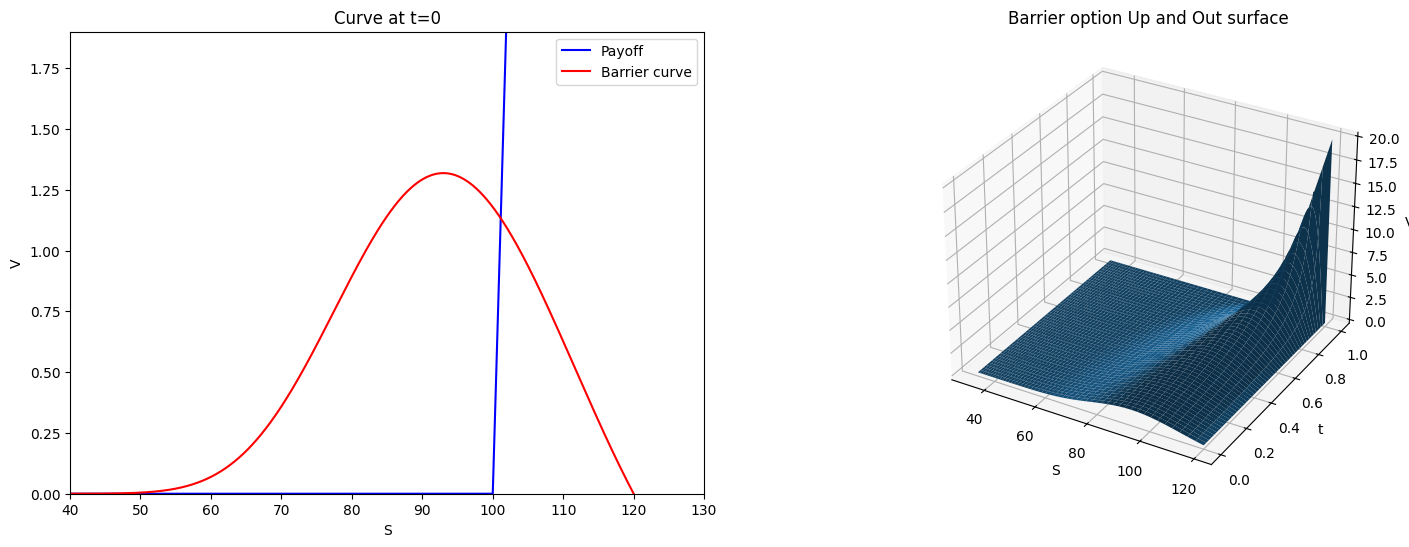
\includegraphics[width=.90\linewidth]{content/images/surface.png}
	\caption{At-the-money up-and-out barrier option}
	\label{fig:surface}
\end{figure}

Figure (\ref{fig:surface}) shows the barrier curve and surface for an at-the-money up-and-out barrier option for $S=100,K=100, T=1, r=10\%,\sigma=20\%, \text{ and }B=120$. The curve assumes the option is close to or at expiration date. As we can see, the option has no value at any price below 100, as the strike price is also 100. However, the call will retain some value, as the option has not reached the barrier of 120. Where the payoff line (blue) and the barrier curve (red) intersects shows the potential payoff at expiration, which is 1.18 according to Black-Scholes.

The surface shows the option value in relation to time and the underlying price. As we can see, the barrier option has the most value when the option is very close to expiration and the stock price is relatively close to the barrier. Otherwise, the option has no value when the underlying is at 40 and the time to expiration is 0. The option also loses it's value when the option is close to the barrier.

    \chapter{Barrier Option Pricing with Monte Carlo}
Suppose the asset price follows a Geometric Brownian Motion (GBM):
\begin{equation}\label{eq:GBM}
	dS_t=rS_tdt+\sigma S_tdW_t
\end{equation}
Where $S_t$ is the asset price at time $t$, $r$ is the risk-free interest rate, $\sigma$ is the volatility of the asset, and $dW_t$ is the increment of a Wiener process. With this process in mind, we can discretize time by dividing the total time into smaller length intervals $\Delta t=T/N.$ Afterwards, we simulate the asset price paths by generating a random standard normal variable $Z$ and using the random variable to update the asset price with the discretized GBM.

\begin{center}
	\begin{table}[H]
    \begin{tabular}{ | m{4em} | m{1.3cm}| m{1.3cm} | m{1.3cm}| m{1.3cm} | m{1.3cm} | m{1.3cm} | m{1.3cm} | m{1.35cm} | m{1.3cm} |} 
  \hline
   & Price & $\text{MC}_{100}$ & $\text{err}_{100}$ & $\text{MC}_{1000}$ & $\text{err}_{1000}$ & $\text{MC}_{5000}$ & $\text{err}_{5000}$ & $\text{MC}_{10000}$ & $\text{err}_{10000}$  \\ 
   \hline
   $S_0=100$ $B=0.01$ &11.1605&10.4632&0.6973&11.4493&-0.2888&10.8657&0.2948&11.1015&0.0590\\
  \hline
  $S_0=100$ $B=95$ & 5.05 & 6.5795 & -1.5295 & 5.8379  & -0.7870 & 5.2264 & -0.1764 & 5.5198 & -0.4698\\ 
  \hline
  $S_0=100$ $B=90$ & 8.5462 & 10.63  & -2.0838 & 9.2705 & -0.7243 & 9.0406 & -0.4944 & 8.9585  & -0.4123\\ 
  \hline 
  $S_0=110$ $B=100$ &11.6763&12.9766&-1.3003&12.5033&-0.8270&12.1231&-0.4468&12.5707&-0.8944 \\
  \hline
  $S_0=110$ $B=90$ &17.7117&15.8569&1.8548&18.5671&-0.8554&18.0540&-0.3423&18.0546&-0.3429\\
  \hline
   $S_0=120$ $B=100$ & 23.4640 & 20.5357  & 2.9283 & 24.9569  & -1.4930 & 24.6213 & -1.1573 & 23.8197 & -0.3557 \\ 
  \hline
  $S_0=120$ $B=110$ & 13.2648 & 18.0740 & -4.8092 & 15.6643 & -2.3995 & 15.3539 & -2.0991 & 15.1735 & -1.9087\\ 
  \hline
\end{tabular}
\caption{MC Down-and-out call with $q=8\%,r=5\%, T=0.5,\sigma=25\%,K=90$}
\label{tab:MC_barrer}
\end{table}
\end{center}
\begin{equation}
	S_{t+\Delta t}=S_t\times\exp\left(\left(r-\frac{\sigma^2}{2}\right)\Delta t+\sigma\sqrt{\Delta t}\times 2\right)
\end{equation}
Table (\ref{tab:MC_barrer}) shows the comparison between the Black-Scholes analytical price and the Monte Carlo simulations for the down-and-out call options. We have chosen options with different Barrier values as well as varying stock values. We've used simulations for $n=100,1000,5000,\text{ and }10000$ and samples.

%    \chapter{Binomial Tree Method}
\label{sec:binomial-tree}

The \textit{binomial tree method} is a widely used approach to price derivative instruments, including barrier options. The method approximates the price evolution of the underlying asset by discretizing time into a finite number of steps, \(N\), between the current time, \(t = 0\), and the maturity, \(T\). The accuracy of the method improves as the number of steps increases, with the binomial tree price converging to the theoretical option price.

\section{Binomial Tree Structure}

A binomial tree models the possible price movements of the underlying asset over time. At each step, the asset price can move either up or down. The price at any node in the tree is calculated using the formula:

\begin{equation}
S_{i,j} = S_0 \cdot u^j \cdot d^{i-j}
\end{equation}

where:
\begin{itemize}
    \item \(S_{i,j}\) is the stock price at step \(i\), level \(j\),
    \item \(S_0\) is the initial stock price,
    \item \(u = e^{\sigma \sqrt{\Delta t}}\) is the up factor,
    \item \(d = \frac{1}{u}\) is the down factor,
    \item \(\Delta t = \frac{T}{N}\) is the time increment per step, and
    \item \(\sigma\) is the volatility of the underlying asset.
\end{itemize}

The risk-neutral probability of an upward movement, \(p\), and a downward movement, \(q\), are defined as:

\begin{equation}
p = \frac{e^{r \Delta t} - d}{u - d}, \quad q = 1 - p
\end{equation}

where \(r\) is the risk-free interest rate.

\section{Example Calculation}

Let us consider an up-and-in European call option with the following parameters:
\begin{itemize}
    \item Spot price (\(S_0\)): 100,
    \item Barrier level (\(B\)): 105,
    \item Strike price (\(K\)): 90,
    \item Risk-free rate (\(r\)): 0.05,
    \item Time to maturity (\(T\)): 1 year,
    \item Volatility (\(\sigma\)): 0.2,
    \item Number of steps (\(N\)): 3.
\end{itemize}

Using these parameters:
\begin{itemize}
    \item The time increment per step is:
    

\[
    \Delta t = \frac{T}{N} = \frac{1}{3} \approx 0.3333 \, \text{years}.
    \]


    \item The up and down factors are:
    

\[
    u = e^{\sigma \sqrt{\Delta t}} = e^{0.2 \sqrt{0.3333}} \approx 1.1224, \quad d = \frac{1}{u} \approx 0.8909
    \]


    \item The risk-neutral probabilities are:
    

\[
    p = \frac{e^{r \Delta t} - d}{u - d} = \frac{e^{0.05 \cdot 0.3333} - 0.8909}{1.1224 - 0.8909} \approx 0.5438, \quad q = 1 - p = 0.4562.
    \]


\end{itemize}

\section{Payoff Calculation}

To calculate the option price, we build the binomial tree and track the stock price at each node. At maturity (\(t = T\)), the payoff for an up-and-in European call option is defined as:

\begin{equation}
\text{Payoff} =
\begin{cases} 
\max(S_T - K, 0), & \text{if } \max(S_t) \geq B \text{ for } t \in [0, T], \\
0, & \text{otherwise.}
\end{cases}
\end{equation}

For the given parameters:
\begin{itemize}
    \item If the stock price reaches or exceeds \(B = 90\) during its lifetime, the payoff is calculated as \(\max(S_T - K, 0)\).
    \item Otherwise, the option expires worthless, with a payoff of 0.
\end{itemize}

\section{Tree Construction and Results}

Figure \ref{fig:binomial-tree} illustrates the binomial tree for the given parameters, showing the possible stock price movements and the resulting option values at each node. The calculated option price, considering the up-and-in barrier condition, is obtained through backward induction along the tree. This ensures that the barrier condition is applied at each step. The final option price is 16.42.


\begin{figure}[h]
    \centering
    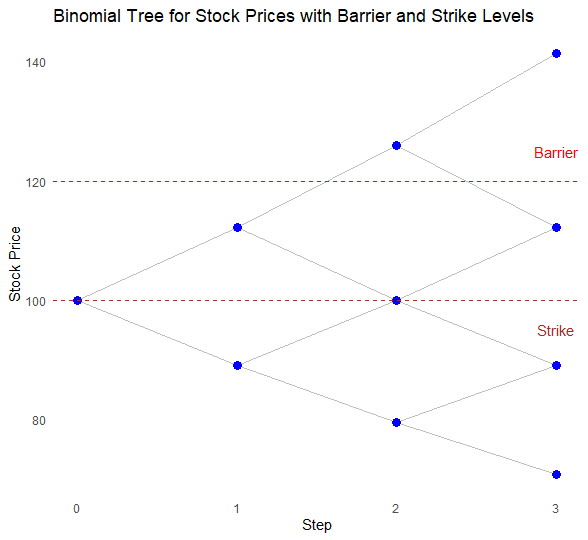
\includegraphics[width=.75\linewidth]{content/images/three-step.png}
    \caption{Binomial Tree with Barrier Level \(B = 90\) and Strike Price \(K = 105\).}
    \label{fig:binomial-tree}
\end{figure}

The binomial tree method provides a flexible and intuitive framework for pricing options, including barrier options. However, as shown in this example, its computational requirements grow significantly with the number of steps \(N\), making it less efficient for path-dependent options. Alternative methods, such as Monte Carlo simulations or analytical solutions, may be more suitable for pricing complex derivatives.

%    \cleardoublepage
    \input{content/chapter-hedging.tex}
	\chapter{The Greeks for Barrier Options}
\label{sec:greeks}

The Greeks are key sensitivities in option pricing that measure how the price of an option changes with respect to various factors such as the underlying asset price, time to maturity, volatility, and interest rates. For barrier options, the calculation of the Greeks is more complex due to the added condition of a barrier, which affects the option's price path and behavior.

For the plots in this section, the parameters are \( S_0 = 40 \), \( K = 50 \), \( T = 1.0 \), \( r = 0.1 \), \( \sigma = 0.2 \), and \( B = 60 \), representing the spot stock price, strike price, time to maturity (in years), risk-free rate, volatility, and barrier level, respectively.




\section{Delta (\(\Delta\))}

Delta for a barrier option measures the sensitivity of the option price to changes in the underlying asset price $S$. It represents the rate of change of the option's price with respect to small changes in the underlying price.
\[
\Delta = \frac{\partial V}{\partial S}
\]

For \textbf{knock-in} barrier options, delta behaves similarly to that of a standard European option but is influenced by the presence of the barrier. It reflects how changes in the underlying price affect the probability of the barrier being breached and the option becoming active. Figure (\ref{fig:delta_upout}) shows the delta behavior of an up-and-out put option as a function of the underlying stock price, $S$. When the stock price is well below the barrier level $B$, delta behaves similarly to a vanilla European put option. As the price approaches the barrier, delta tends toward zero because the likelihood of the option being knocked out increases, reducing its sensitivity.

To further analyze the delta across different barrier options, refer to the table below:
\begin{center}
	\begin{table}[H]
		\begin{tabular}{ | m{3cm} | m{5cm}| m{4cm} | m{4cm}|} 
			\hline
			\textbf{Barrier Type} & \textbf{Price Far from Barrier} & \textbf{Price Near the Barrier} & \textbf{Intuition}  \\
			\hline
			\textbf{Knock-Out} & Similar to vanilla options     & $\Delta \to 0$ as $S \to B$  & Probability of knock-out increases as $S$ nears $B$. \\ 
			\hline
			\textbf{Knock-In}  & $\Delta \approx 0$ far from barrier   & $\Delta \uparrow$ as $S \to B$  & Option becomes active as the price hits the barrier. \\ 
			\hline
		\end{tabular}
		\caption{Delta behavior for different types of barrier options.}
		\label{tab:delta_barrier_options}
	\end{table}
\end{center}
\textbf{Key Intuition:}
\begin{itemize}
	\item \textbf{Knock-Out Options:} Lose their sensitivity as $\Delta$ tends toward $0$ as the likelihood of being knocked out near the barrier increases.
	\item \textbf{Knock-In Options:} Show increasing sensitivity as the underlying price nears the barrier because the probability of activation rises.
\end{itemize}

The visual analysis in Figure (\ref{fig:delta_upout}) shows delta behavior for an up and out put option. The insights from the plot matches the intuition from Table (\ref{tab:delta_barrier_options}) which provides a comprehensive understanding of how delta behaves across different types of barrier options. Before the stock price hits the barrier, the delta is similar to one of a vanilla option. As the stock price hits the barrier, there is a steep decline in delta as the option is knocked out and the option price is zero.
\begin{figure}[H]
    \centering
    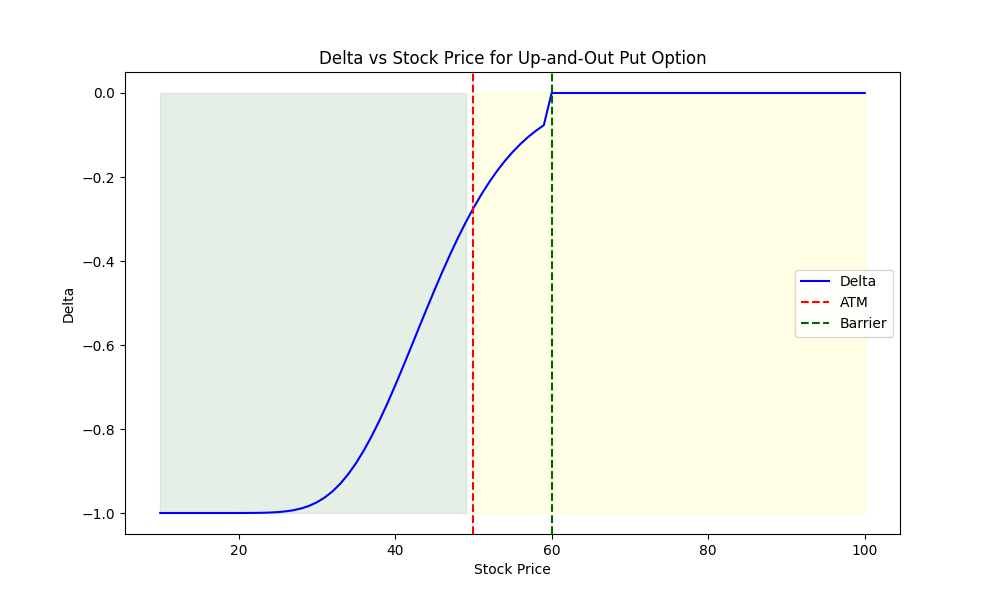
\includegraphics[width=.65\linewidth]{content/images/delta.png}
    \caption{Delta of up-and-out Put Option vs. the Stock Price.}
    \label{fig:delta_upout}
\end{figure}

\subsection{Delta Hedging}

In this section, we retrieve NVDA prices from October 21--25, 2024, using the parameters \( K = 143 \), \( T = 1 \), \( r = 0.046 \), \( \sigma = 0.5 \), and \( B = 150 \), which represent the strike price, time to maturity, risk-free rate, volatility, and barrier level, respectively. We calculated the option price and its delta. The unhedged and hedged changes are presented in Table (\ref{tab:hedging}), demonstrating the effectiveness of delta hedging in minimizing investment risks. Figure (\ref{fig:hedgingvunhedging}) provides a visual comparison of hedged versus unhedged changes from October 22 to 24, 2024; illustrating that hedging reduces risk by minimizing the volatility of the option price.

\begin{table}[h]
    \centering
    \caption{Option Pricing and Delta Hedging}
    \label{tab:hedging}
    \begin{tabular}{|c|c|c|c|c|c|}
        \hline
        \textbf{Date} & \textbf{Stock Price} & \textbf{Option Price} & \textbf{Delta} & \textbf{Unhedged Change} & \textbf{Hedged Change} \\
        \hline
        October 21 & 143.71 & 24.23653 & -0.3624546 & NA & NA \\
        \hline
        October 22 & 143.59 & 24.28006 & -0.3630813 & 0.04353214 & $3.759243 \times 10^{-5}$ \\
        \hline
        October 23 & 139.56 & 25.78639 & -0.3846464 & 1.50633247 & $4.311500 \times 10^{-2}$ \\
        \hline
        October 24 & 140.41 & 25.46142 & -0.3800139 & -0.32497748 & $1.971995 \times 10^{-3}$ \\
        \hline
        October 25 & 141.54 & 25.03545 & -0.3739251 & -0.42596805 & $3.447701 \times 10^{-3}$ \\
        \hline
    \end{tabular}
\end{table}

\begin{figure}[h]
    \centering
    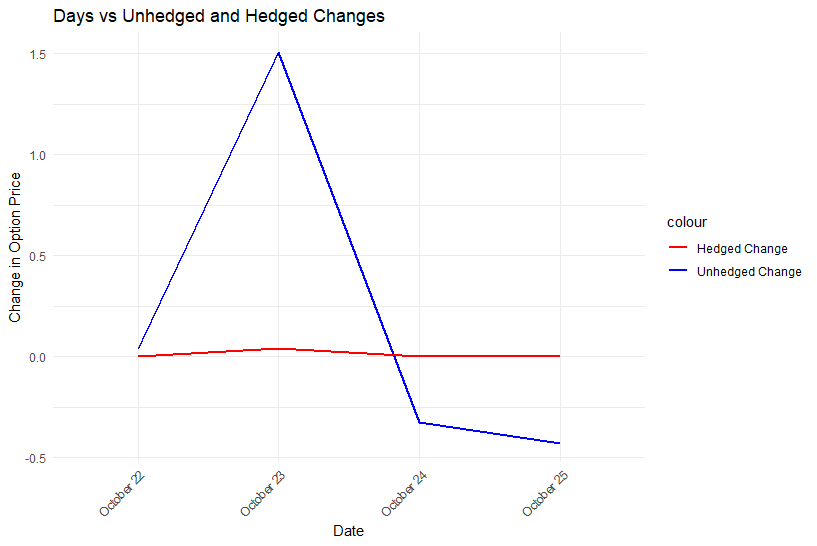
\includegraphics[width=0.65\linewidth]{content/images/hedgedvsunhedged.png}
    \caption{Comparison of change in Option Price of a hedged investment vs unhedged investment}
    \label{fig:hedgingvunhedging}
\end{figure}

\section{Gamma (\(\Gamma\))}

Gamma (\(\Gamma\)) for a barrier option measures the rate of change of delta (\(\Delta\)) with respect to changes in the underlying asset price (\(S\)). It represents the curvature or sensitivity of delta in response to movements in the underlying price. It provides insights into how rapidly an option's delta will change as the underlying price fluctuates.
\[
\Gamma = \frac{\partial^2 V}{\partial S^2}
\]

For \textbf{knock-in} and \textbf{knock-out} barrier options, gamma exhibits unique behavior due to the presence of the barrier. The interaction between the price of the stock, the barrier level and the time to maturity influences how gamma behaves in different scenarios.

\begin{center}
	\begin{table}[H]
		\begin{tabular}{ | m{3cm} | m{5cm}| m{4cm} | m{4cm}|} 
			\hline
			\textbf{Barrier Type} & \textbf{Price Far from Barrier} & \textbf{Price Near the Barrier} & \textbf{Intuition}  \\ 
			\hline
			\textbf{Knock-Out} & Similar to vanilla options     & $\Gamma \uparrow$ as $S \to B$  & Gamma spikes as the price nears the barrier due to increased risk of knock-out. \\ 
			\hline
			\textbf{Knock-In}    & $\Gamma \approx 0$ far from barrier   & $\Gamma \uparrow$ as $S \to B$  & Gamma rises as the stock price approaches the barrier due to increased probability of activation. \\ 
			\hline
		\end{tabular}
		\caption{Gamma behavior for Knock-In and Knock-Out barrier options.}
		\label{tab:gamma_barrier_options}
	\end{table}
\end{center}

Figure (\ref{fig:gamma_behavior}) illustrates the gamma behavior of an up-and-out put option as a function of the underlying stock price (\(S\)). As soon as the barrier is hit, the option is knocked out and gamma goes to zero. Gamma hedging is a risk management strategy used in options trading to mitigate the risks associated with large movements in the underlying asset's price. These large movements may cause large losses in delta hedged portfolio. Figure \ref{fig:compare_deltagamma_hedge} shows that hedging both delta and gamma provides minimum risk investment.

\begin{figure}[h]
    \centering
    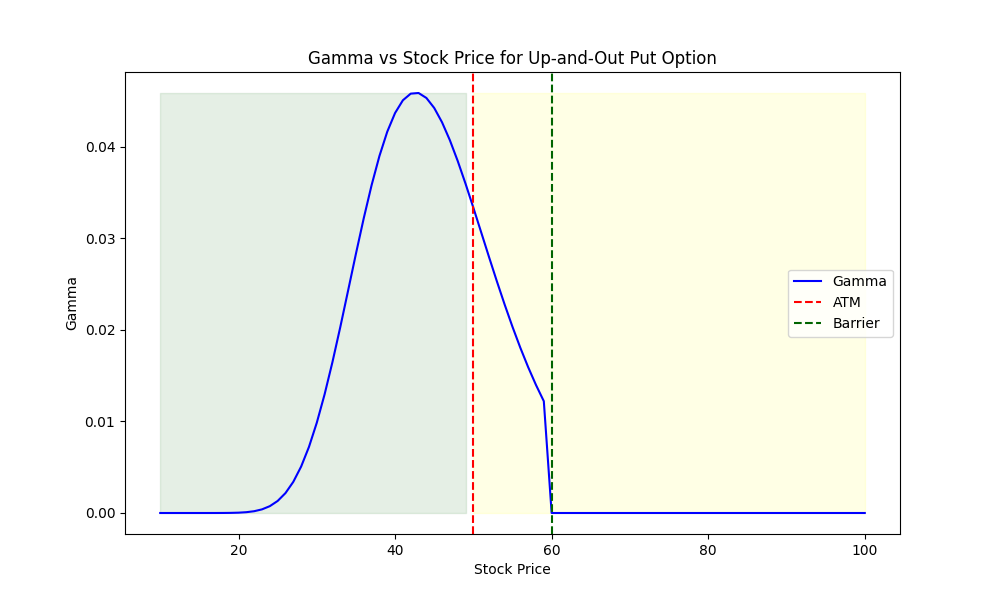
\includegraphics[width=.65\linewidth]{content/images/gamma.png}
    \caption{Gamma of an up-and-out put option vs. the Stock Price.}
    \label{fig:gamma_behavior}
\end{figure}

\begin{figure}[h]
    \centering
    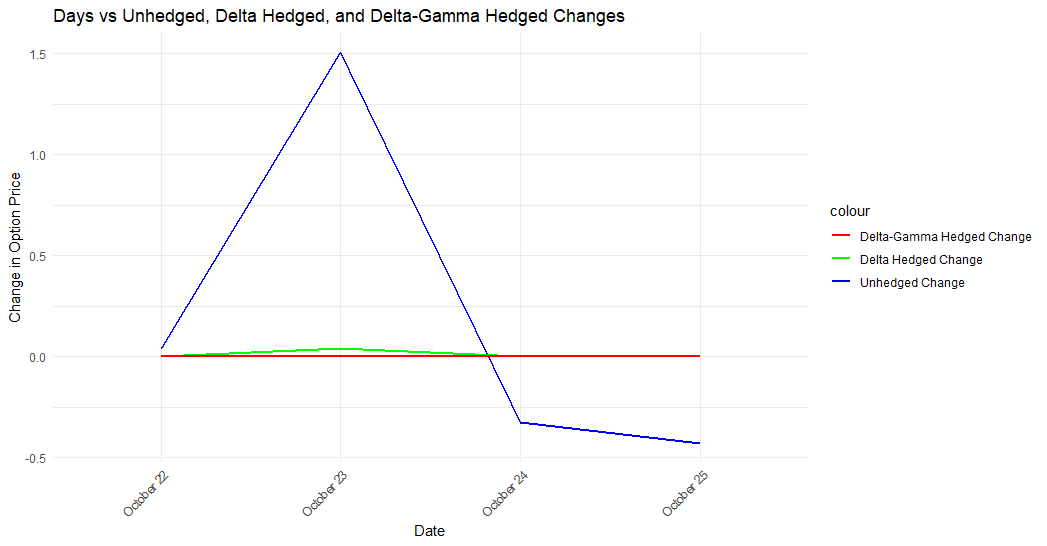
\includegraphics[width=.65\linewidth]{content/images/compare_hedging.png}
    \caption{Comparing different hedging results}
    \label{fig:compare_deltagamma_hedge}
\end{figure}


\begin{figure}[h]
    \centering
    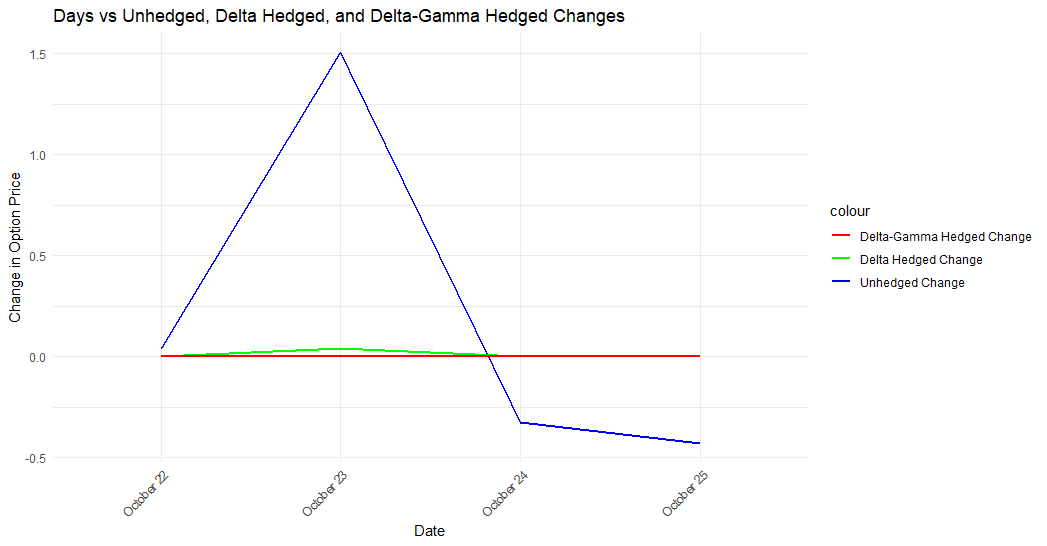
\includegraphics[width=.65\linewidth]{content/images/compare_hedging.png}
    \caption{Comparing different hedging results}
    \label{fig:compare_deltagamma_hedge}
\end{figure}


\begin{figure}[h]
	\centering
	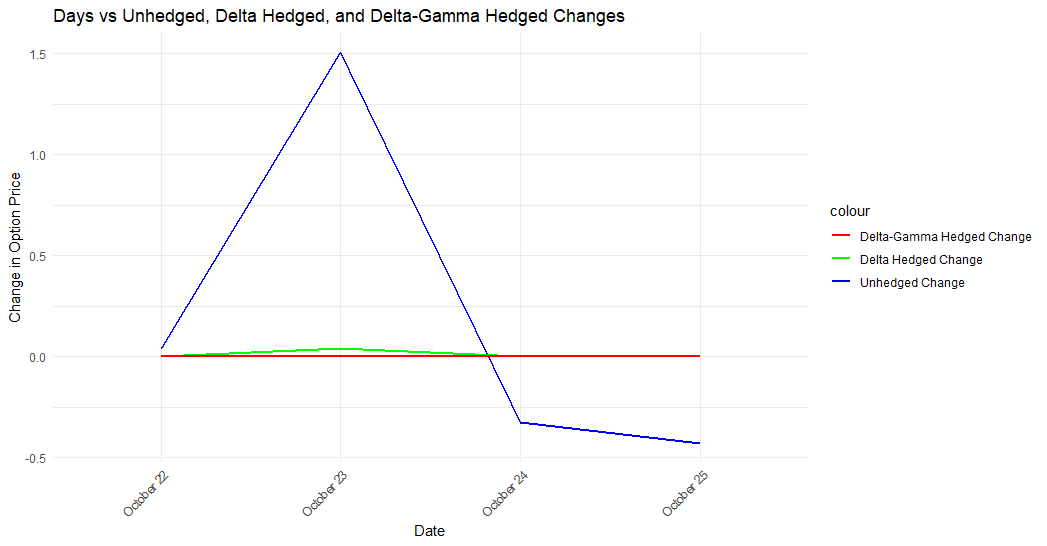
\includegraphics[width=.65\linewidth]{content/images/compare_hedging.png}
	\caption{Comparing different hedging results}
	\label{fig:compare_deltagamma_hedge}
\end{figure}


\section{Vega ($\nu$)}

Vega, $\nu$, measures the sensitivity of the option price to changes in volatility. For barrier options, the calculation of vega incorporates adjustments to account for the probability of breaching the barrier level under varying volatility conditions.
\[
\nu = \frac{\partial V}{\partial \sigma}
\]

\begin{itemize}
	\item \textbf{Knock-In Options:} Increased volatility raises the likelihood of the underlying asset price crossing the barrier level, making the option more valuable. As a result, \(\nu\) (vega) will generally be positive.
	\item \textbf{Knock-Out Options:} Increased volatility can lead to a higher probability of the option being knocked out, reducing its value. Therefore, \(\nu\) will tend to be negative for these types of options.
\end{itemize}

\begin{figure}[H]
    \centering
    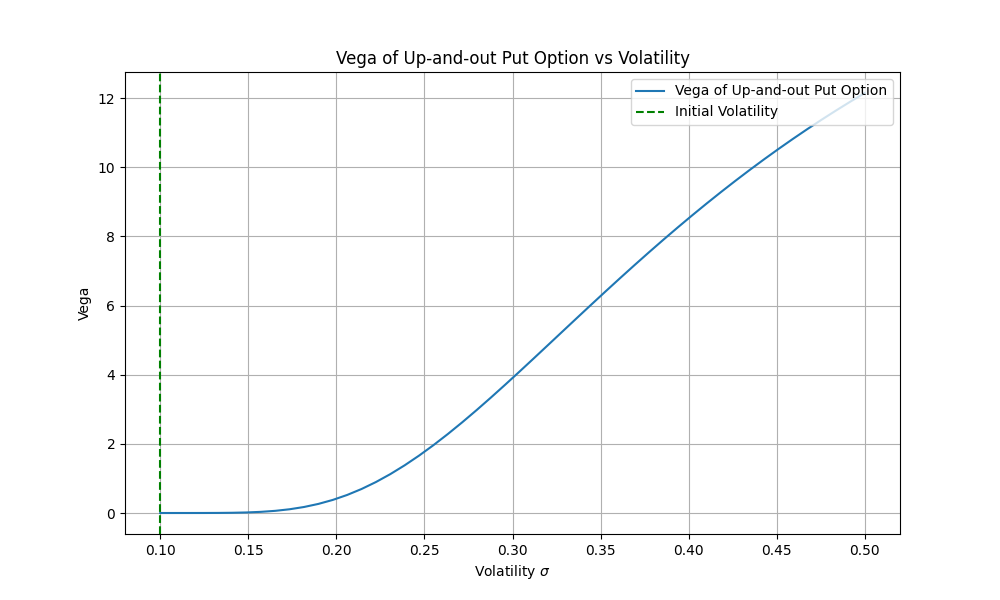
\includegraphics[width=.65\linewidth]{content/images/vega_upout.png}
    \caption{Vega vs Stock Price of an Up-and-Out Put Option}
    \label{fig:vega_behavior}
\end{figure}

The visualization shown in Figure (\ref{fig:vega_behavior}) provides insights into how Vega behaves with changes in stock price across up-and-out put option. The sensitivity patterns are influenced by the interplay between volatility and the probability of breaching the barrier level. As the barrier is breached, vega immediately goes to zero.

\section{Theta ($\Theta$)}

Theta, $\Theta$, measures the rate of change of an option's price with the passage of time, assuming all other variables remain constant. It is a critical "Greek" that reflects time decay, which is the gradual erosion of the option's value as expiration approaches. In the case of barrier options, theta is influenced not only by the time remaining but also by the interaction with the barrier level and the path dependency of the option.

Barrier options are unique because their payoff depends on the underlying asset price crossing (or not crossing) a specified barrier level during the option's lifetime. As such, the sensitivity of theta changes depending on proximity to the barrier, time remaining until maturity, and whether the option is near the knock-in or knock-out condition.

\begin{itemize}
    \item \textbf{Knock-In Options:} As time to maturity decreases, the value of knock-in options tends to decline, especially when the underlying asset price is far from the barrier. This is because the likelihood of triggering the option by crossing the barrier becomes lower as time runs out.
    
    \item \textbf{Knock-Out Options:} As time to maturity approaches, the risk of the underlying price reaching the barrier and knocking out the option increases, thereby accelerating time decay.
\end{itemize}


\begin{figure}[H]
    \centering
    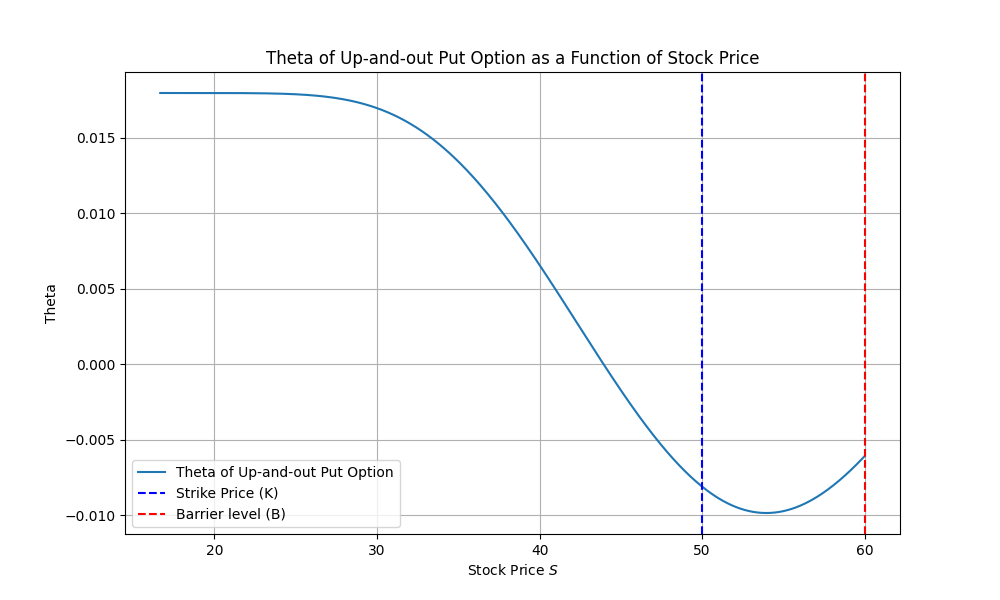
\includegraphics[width=.65\linewidth]{content/images/theta.png}
    \caption{Theta vs Stock Price of an Up-and-Out Put Option}
    \label{fig:theta_behavior}
\end{figure}


The visualization in Figure (\ref{fig:theta_behavior}) illustrates the relationship between stock price and theta for an up-and-out put option. This analysis highlights how theta's sensitivity varies depending on proximity to the barrier. As the stock price approaches the strike, theta is decreasing. As the stock price approaches the barrier, it is increasing. However, when stock price hits the barrier, theta immediately goes to zero.


\section{Rho (\(\rho\))}

Rho, $\rho$, for barrier options measures the sensitivity of the option price to changes in the risk-free interest rate (\(r\)). It represents how much the value of the option changes when the risk-free rate changes by 1\%. Rho is important in understanding the impact of monetary policy, such as changes in interest rates, on the value of barrier options.

\[
\rho = \frac{\partial V}{\partial r}
\]

When interest rates rise:
\begin{itemize}
	\item \textbf{Knock-In Options:} Tend to show a positive relationship with Rho (\(\rho\)). This reflects that higher interest rates increase the present value of the potential payoff, making the knock-in option more valuable.
	\item \textbf{Knock-Out Options:} Tend to show muted sensitivity to changes in the interest rate. This is because the likelihood of being knocked out (and thus losing value) dominates any benefit gained from higher interest rates.
\end{itemize}
\begin{figure}[H]
    \centering
    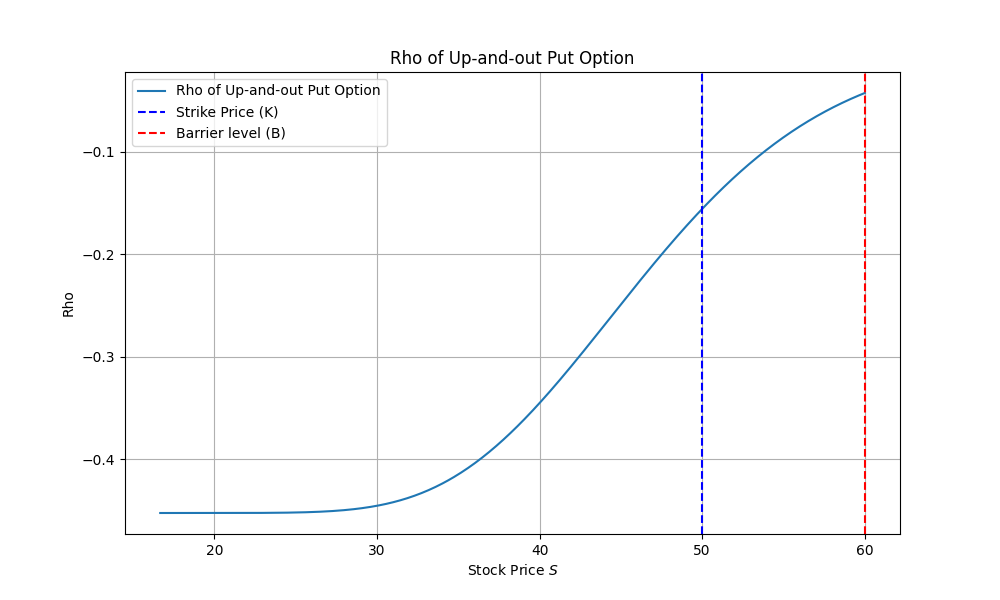
\includegraphics[width=.65\linewidth]{content/images/rho.png}
    \caption{Rho vs Stock Price for an Up-and-Out Put Option}
    \label{fig:rho_behavior}
\end{figure}

The visual behavior in Figure~\ref{fig:rho_behavior} illustrates how changes in the stock price (\(r\)) impact rho of an up-and-out barrier option. As the stock price increase, rho also increases. However, as stock price breaches the barrier, rho goes to zero.
	
\bibliographystyle{plainnat}
\begin{thebibliography}{9}
	\bibitem{JohnRubinstein1985}
	Cox, John C. "Options Markets." (1985).
\end{thebibliography}

	\cleardoublepage
	\begin{appendices}
\chapter{Formulas and Proofs}
\section{Black-Scholes PDE for Barrier Options}
\label{section:A1}
\newpage
\section{Payoffs Formulas for Single Barrier Options}
\label{section:A2}
The formula for Single Barrier options have been proved by Reiner and Rubinstein. The payoff of a Single Barrier call or put depends on the following formulas:
\[
\begin{aligned}
	A_1&=Se^{-q\tau}aN(ax_1)-Ke^{-r\tau}N(ax_1-a\sigma\sqrt{\tau})\\
	A_2&=Se^{-q\tau}aN(ax_1)-Ke^{-r\tau}N(ax_2-a\sigma\sqrt{\tau})\\
	A_3&=Se^{-q\tau}a\left(\tfrac{B}{S}\right)^{2\lambda+2}N(bx_3)-K\left(\tfrac{B}{S}\right)^{2\lambda}e^{-r\tau}N(bx_3-b\sigma\sqrt{\tau})\\
	A_4&=Se^{-q\tau}a\left(\tfrac{B}{S}\right)^{2\lambda+2}N(bx_4)-K\left(\tfrac{B}{S}\right)^{2\lambda}e^{-r\tau}N(bx_4-b\sigma\sqrt{\tau})\\
	A_5&=Ke^{-rT}\left[N(bx_2-b\sigma\sqrt{\tau})-\left(\tfrac{B}{S}\right)^{2\lambda}N\left(bx_4-b\sigma\sqrt{\tau}\right)\right]\\
	A_6&=Ke^{-rT}\left[N(bx_5-b\sigma\sqrt{\tau})-\left(\tfrac{B}{S}\right)^{2\lambda}N\left(bx_5-b\sigma\sqrt{\tau}\right)\right]
\end{aligned}
\]
with
\[
\begin{cases}
	a=1,-1&\text{call or put}\\
	b=1,-1&\text{out or in}
\end{cases}
\]
where $x_1,x_2,x_3,x_4,x_5$ is the following:
\[
\begin{aligned}
	&x_1=\frac{\ln\left(\frac{S}{K}\right)}{\sigma\sqrt{\tau}}+(1+\mu)\sigma\sqrt{\tau},\quad x_2=\frac{\ln\left(\frac{S}{B}\right)}{\sigma\sqrt{\tau}}+(1+\mu)\sigma\sqrt{\tau}\\
	&x_3=\frac{\ln\left(\frac{B^2}{SK}\right)}{\sigma\sqrt{\tau}}+(1+\mu)\sigma\sqrt{\tau},\quad x_4=\frac{\ln\left(\frac{B}{S}\right)}{\sigma\sqrt{\tau}}+(1+\mu)\sigma\sqrt{\tau}\\
	x_5=\frac{\ln\left(\frac{B}{S}\right)}{\sigma\sqrt{\tau}}+\lambda\sigma\sqrt{\tau}
\end{aligned}
\]
where $\mu$ and $\lambda$ is the following
\[
\mu=\frac{r-q-\tfrac{\sigma^2}{2}}{\sigma^2},\quad\lambda=\sqrt{\mu^2+\frac{2q}{\sigma^2}}
\]
\end{appendices}


	
	% --------------------------
	% Back matter
	% --------------------------
	%{%
		%	\setstretch{1.1}
		%	\renewcommand{\bibfont}{\normalfont\small}
		%	\setlength{\biblabelsep}{0pt}
		%	\setlength{\bibitemsep}{0.5\baselineskip plus 0.5\baselineskip}
		%	\printbibliography[nottype=online]
		%	\printbibliography[heading=subbibliography,title={Webseiten},type=online,prefixnumbers={@}]
		%}
	
%	\listoffigures
	
%	\listoftables
%	\cleardoublepage


	
	
	
	% **************************************************
	% End of Document CONTENT
	% **************************************************
\end{document}
